\section{Polarización de la juntura BE}
En cualquiera de las aplicaciones en las que se usa el transistor, sea como amplificador o
dispositivo de conmutación, se requiere la polarización en directa de la juntura base-emisor.
En esta parte del práctico se propuso caracterizar el comportamiento de la juntura en cuestión.

\subsection{Actividad de laboratorio}

\begin{table}[h!]
\centering
\begin{tabular}{|c|c|c|c|c|c|c|}
\hline
$V_{BB}$ & 500\,mV & 1\,V & 2\,V & 3\,V & 4\,V & 10\,V \\
\hline
$I_B$ (mA) & 1 & 3{,}4 & 14 & 23{,4} & 33 & 91{,}4 \\
\hline
$V_{BE}$ (mV) & 430 & 540 & 640 & 670 & 690 & 740 \\
\hline
\end{tabular}
\caption{Ejemplo de la tabla a confeccionar.}
\end{table}

\begin{figure}[h!]
\centering
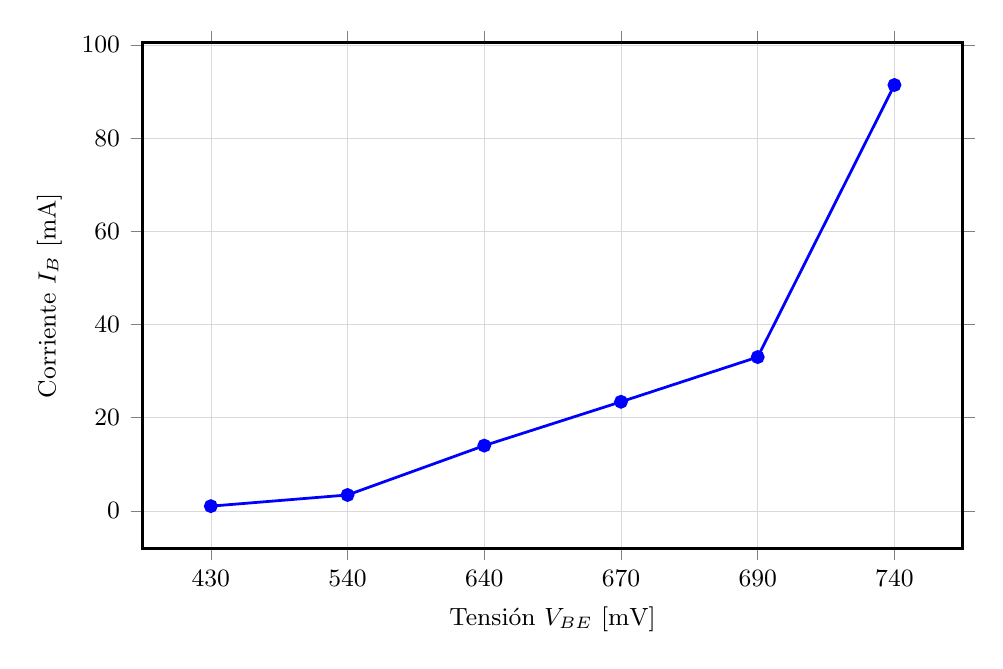
\begin{tikzpicture}
\begin{axis}[
    width=12cm,
    height=8cm,
    grid=both,
    xlabel={Tensión $V_{BE}$ [mV]},
    ylabel={Corriente $I_B$ [mA]},
    xtick=data,
    xticklabels={430, 540, 640, 670, 690, 740},
    enlarge x limits=0.1,
    ytick={0, 20, 40, 60, 80, 100},
    tick label style={font=\small},
    label style={font=\small},
    title style={font=\small},
    legend style={font=\small},
    tick align=outside,
    major grid style={line width=0.2pt, draw=gray!30},
    line width=1pt,
    mark size=2pt
]
\addplot[
    color=blue,
    mark=*,
    line width=1pt
]
coordinates {
    (0, 1)
    (1, 3.4)
    (2, 14)
    (3, 23.4)
    (4, 33)
    (5, 91.4)
};
\end{axis}
\end{tikzpicture}
\caption{Gráfica de $I_B$ en función de $V_{BE}$ con separación equidistante en el eje horizontal.}
\end{figure}

/////////
insertar imágenes y la conclusión
///////


\subsection{Conclusión}


\newpage
